% Gráficos TikZ para Análise Estatística Descritiva
% Baseado na análise dos 179 artigos consolidados

\documentclass{standalone}
\usepackage{pgfplots}
\usepackage{tikz}
\pgfplotsset{compat=1.18}

\begin{document}

% Gráfico 1: Distribuição Temporal (2015-2025)
\begin{figure}
\centering
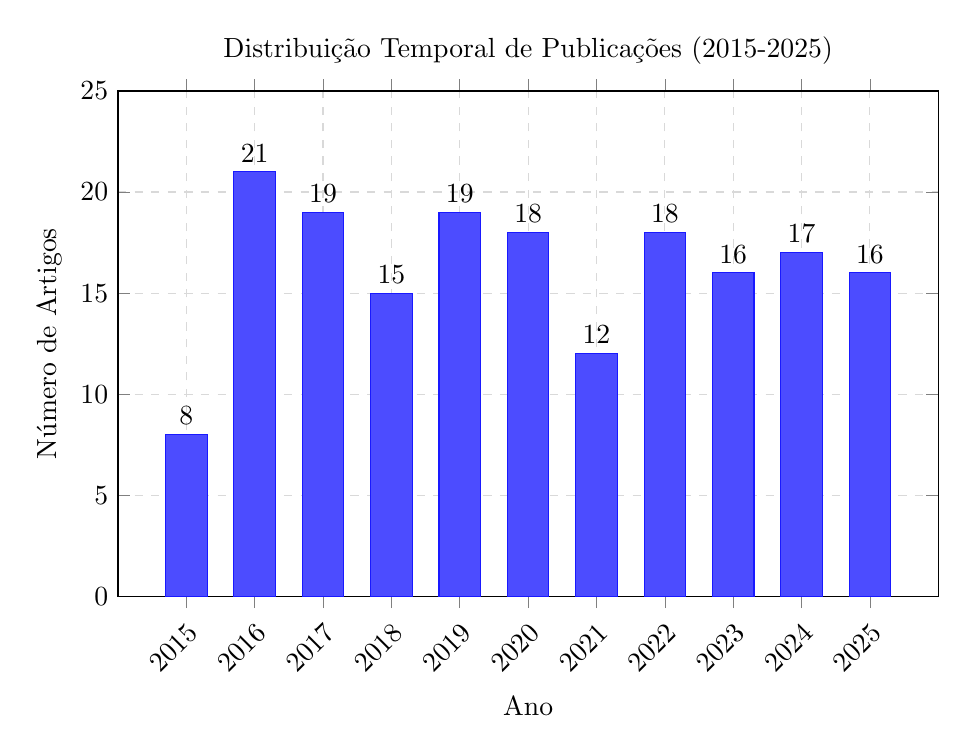
\begin{tikzpicture}
\begin{axis}[
    title={Distribuição Temporal de Publicações (2015-2025)},
    xlabel={Ano},
    ylabel={Número de Artigos},
    width=12cm,
    height=8cm,
    ybar,
    bar width=15pt,
    ymin=0,
    ymax=25,
    symbolic x coords={2015,2016,2017,2018,2019,2020,2021,2022,2023,2024,2025},
    xtick=data,
    xticklabel style={rotate=45, anchor=north east},
    nodes near coords,
    grid=major,
    grid style={dashed,gray!30},
]
\addplot[fill=blue!70, draw=blue!90] coordinates {
    (2015,8) (2016,21) (2017,19) (2018,15) (2019,19)
    (2020,18) (2021,12) (2022,18) (2023,16) (2024,17) (2025,16)
};
\end{axis}
\end{tikzpicture}
\caption{Evolução temporal das publicações sobre tecnologias de avaliação em PBL}
\label{fig:temporal}
\end{figure}

% Gráfico 2: Categorização Tecnológica (Top 8)
\begin{figure}
\centering
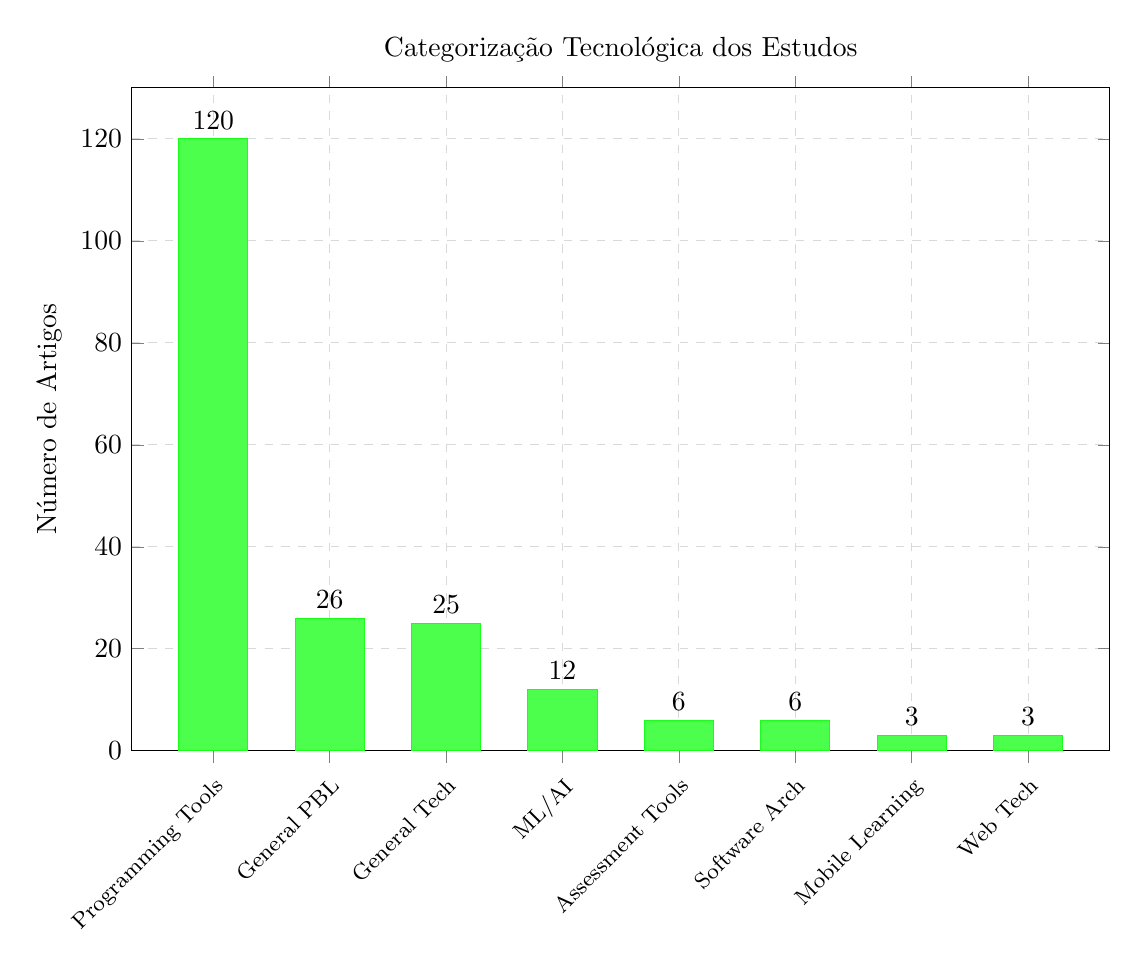
\begin{tikzpicture}
\begin{axis}[
    title={Categorização Tecnológica dos Estudos},
    ylabel={Número de Artigos},
    width=14cm,
    height=10cm,
    ybar,
    bar width=25pt,
    ymin=0,
    ymax=130,
    symbolic x coords={Programming Tools, General PBL, General Tech, ML/AI, Assessment Tools, Software Arch, Mobile Learning, Web Tech},
    xtick=data,
    xticklabel style={rotate=45, anchor=north east, font=\footnotesize},
    nodes near coords,
    grid=major,
    grid style={dashed,gray!30},
]
\addplot[fill=green!70, draw=green!90] coordinates {
    ({Programming Tools},120) ({General PBL},26) ({General Tech},25) ({ML/AI},12)
    ({Assessment Tools},6) ({Software Arch},6) ({Mobile Learning},3) ({Web Tech},3)
};
\end{axis}
\end{tikzpicture}
\caption{Distribuição dos estudos por categoria tecnológica}
\label{fig:tecnologia}
\end{figure}

% Gráfico 3: Lacunas Tecnológicas (Tecnologias Emergentes)
\begin{figure}
\centering
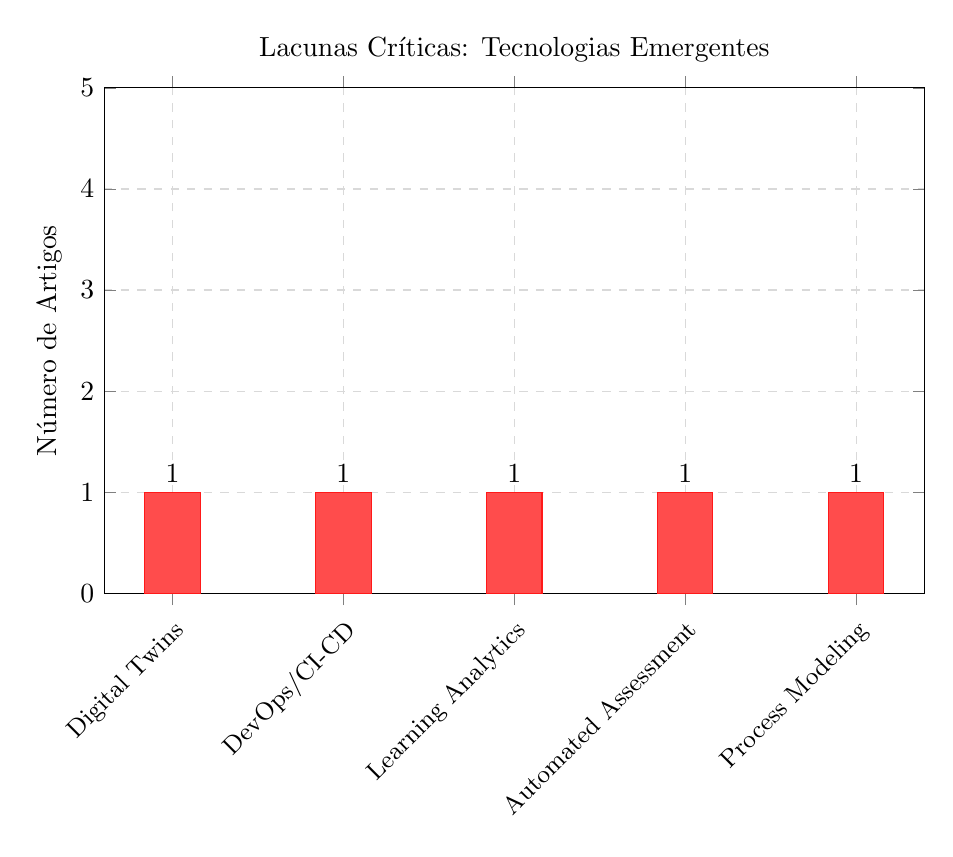
\begin{tikzpicture}
\begin{axis}[
    title={Lacunas Críticas: Tecnologias Emergentes},
    ylabel={Número de Artigos},
    width=12cm,
    height=8cm,
    ybar,
    bar width=20pt,
    ymin=0,
    ymax=5,
    symbolic x coords={Digital Twins, DevOps/CI-CD, Learning Analytics, Automated Assessment, Process Modeling},
    xtick=data,
    xticklabel style={rotate=45, anchor=north east, font=\small},
    nodes near coords,
    grid=major,
    grid style={dashed,gray!30},
]
\addplot[fill=red!70, draw=red!90] coordinates {
    ({Digital Twins},1) ({DevOps/CI-CD},1) ({Learning Analytics},1) 
    ({Automated Assessment},1) ({Process Modeling},1)
};
\end{axis}
\end{tikzpicture}
\caption{Identificação de lacunas críticas em tecnologias emergentes}
\label{fig:lacunas}
\end{figure}

% Gráfico 4: Tipos de Avaliação
\begin{figure}
\centering
\begin{tikzpicture}
\begin{axis}[
    title={Distribuição por Tipos de Avaliação},
    width=12cm,
    height=8cm,
    ybar horizontal,
    bar width=15pt,
    xmin=0,
    xmax=110,
    symbolic y coords={Portfolio, Project, Automated, Self, Peer, Summative, Formative, General},
    ytick=data,
    nodes near coords,
    nodes near coords align={horizontal},
    grid=major,
    grid style={dashed,gray!30},
]
\addplot[fill=orange!70, draw=orange!90] coordinates {
    (2,{Portfolio}) (4,{Project}) (6,{Automated}) (13,{Self})
    (14,{Peer}) (21,{Summative}) (38,{Formative}) (104,{General})
};
\end{axis}
\end{tikzpicture}
\caption{Tipos de avaliação abordados nos estudos}
\label{fig:avaliacao}
\end{figure}

% Gráfico 5: Distribuição Geográfica (Top 6)
\begin{figure}
\centering
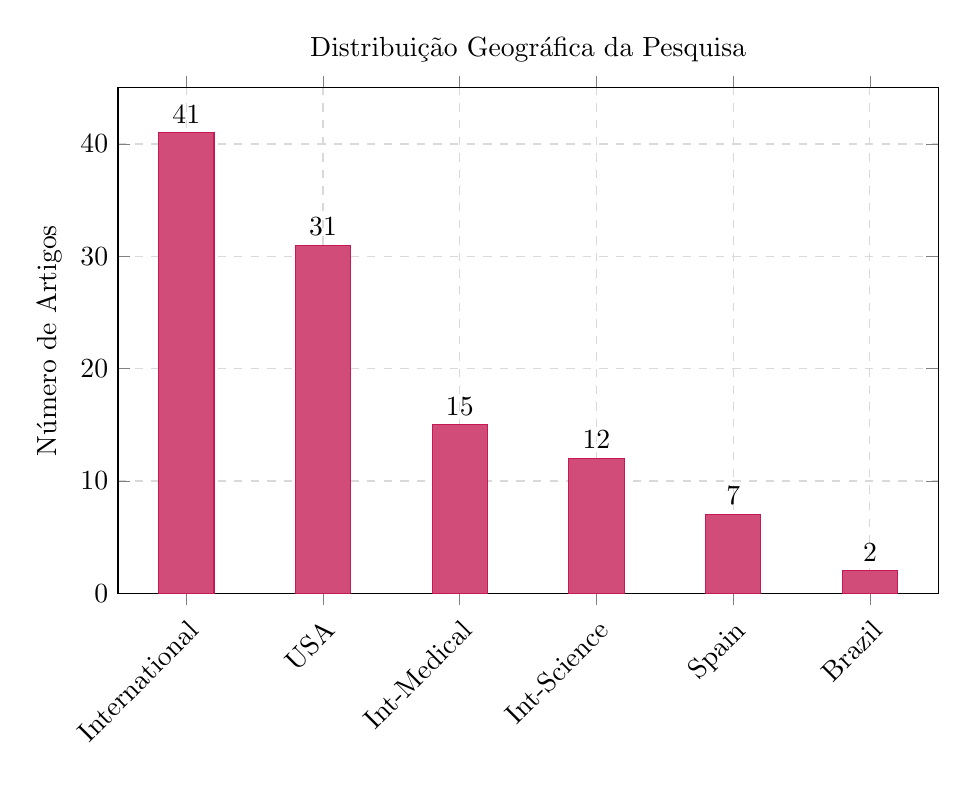
\begin{tikzpicture}
\begin{axis}[
    title={Distribuição Geográfica da Pesquisa},
    ylabel={Número de Artigos},
    width=12cm,
    height=8cm,
    ybar,
    bar width=20pt,
    ymin=0,
    ymax=45,
    symbolic x coords={International, USA, Int-Medical, Int-Science, Spain, Brazil},
    xtick=data,
    xticklabel style={rotate=45, anchor=north east},
    nodes near coords,
    grid=major,
    grid style={dashed,gray!30},
]
\addplot[fill=purple!70, draw=purple!90] coordinates {
    (International,41) (USA,31) ({Int-Medical},15) 
    ({Int-Science},12) (Spain,7) (Brazil,2)
};
\end{axis}
\end{tikzpicture}
\caption{Principais regiões/países produtores de pesquisa}
\label{fig:geografica}
\end{figure}

% Gráfico 6: Tendência de Gêmeos Digitais vs Outras Tecnologias
\begin{figure}
\centering
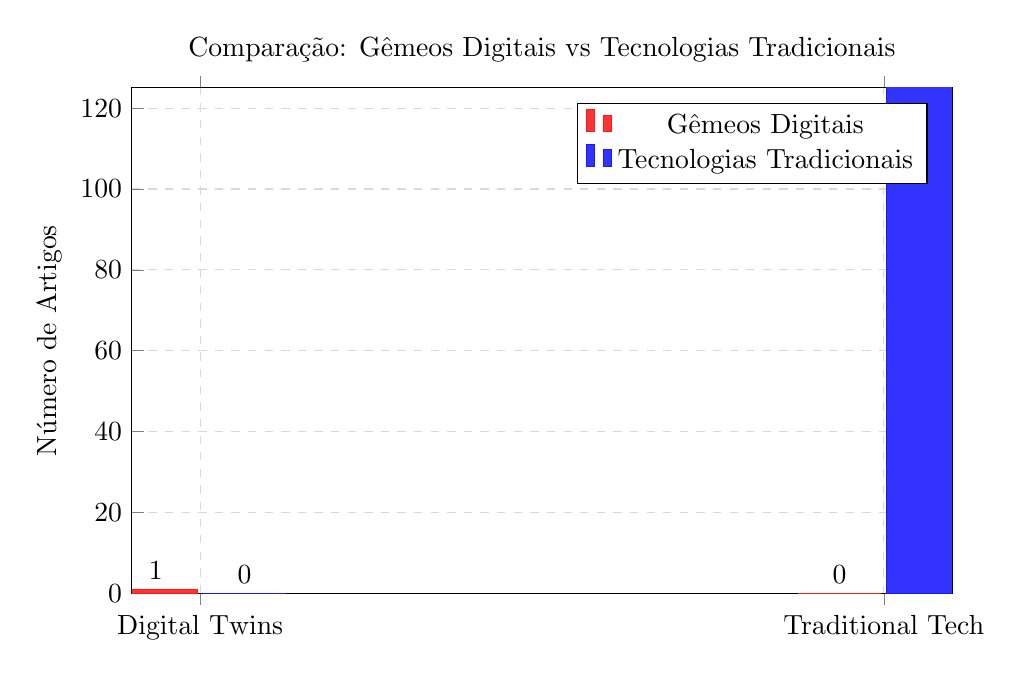
\begin{tikzpicture}
\begin{axis}[
    title={Comparação: Gêmeos Digitais vs Tecnologias Tradicionais},
    ylabel={Número de Artigos},
    width=12cm,
    height=8cm,
    ybar,
    bar width=30pt,
    ymin=0,
    ymax=125,
    symbolic x coords={Digital Twins, Traditional Tech},
    xtick=data,
    nodes near coords,
    grid=major,
    grid style={dashed,gray!30},
    legend entries={Gêmeos Digitais, Tecnologias Tradicionais},
    legend pos=north east,
]
\addplot[fill=red!80, draw=red!90] coordinates {
    ({Digital Twins},1) ({Traditional Tech},0)
};
\addplot[fill=blue!80, draw=blue!90] coordinates {
    ({Digital Twins},0) ({Traditional Tech},178)
};
\end{axis}
\end{tikzpicture}
\caption{Lacuna massiva: Gêmeos Digitais vs Tecnologias Tradicionais}
\label{fig:gemeos}
\end{figure}

\end{document}